\documentclass[../main.tex]{subfiles}
\begin{document}


\section{Neuronale Netze}

\begin{figure}[h!]
  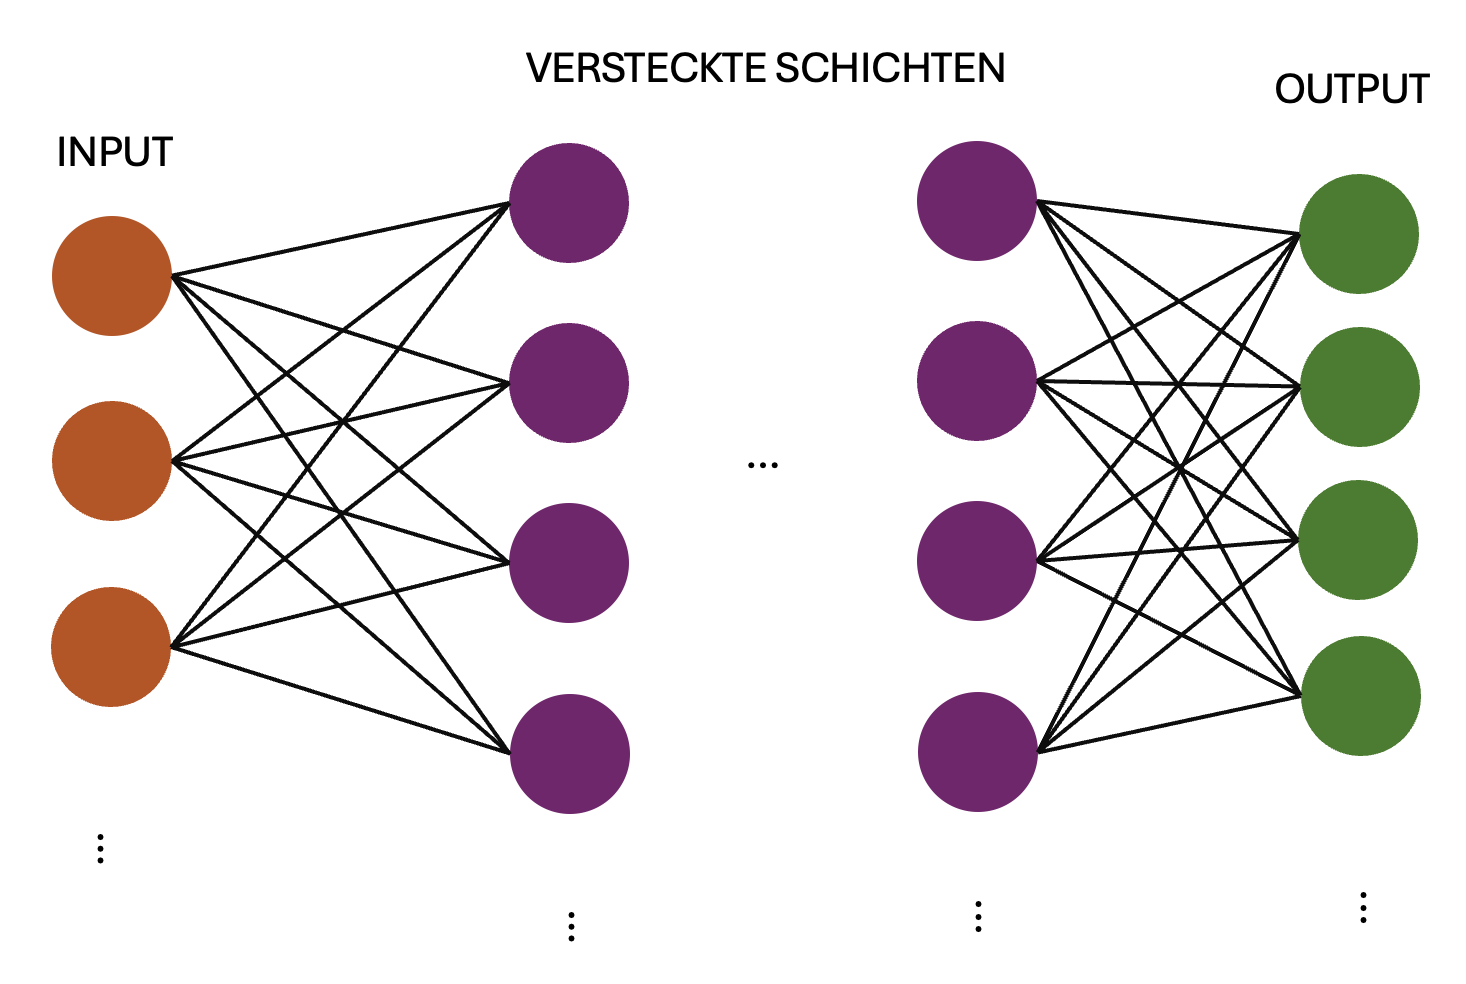
\includegraphics[scale=0.6]{bilder/NeuralNetwork.png}
  \caption{Neuronales Netzwerk}
  \label{fig:NN}
\end{figure}

\glspl{nn} bilden die Basis für \glslink{glos:ki}{KI} und sind in ihrer Funktionsweise dem menschlichen Gehirn nachempfunden. Sie bestehen aus einer Anzahl von Neuronen, die – wie in Abb. \ref{fig:NN} dargestellt – in verschiedenen Schichten angeordnet sind. Die erste Schicht heißt Eingabeschicht, die letzte Ausgabeschicht, dazwischen liegen sogenannte versteckte Schichten. Jedes Neuron ist über gewichtete Verbindungen mit allen Neuronen der vorherigen und nachfolgenden Schicht verbunden. Ein Neuron nimmt zu jedem Zeitpunkt einen Wert zwischen 0 und 1 an, welcher der Ausgabe des Neurons entspricht. Dieser Wert wird aus der Verarbeitung der Eingaben errechnet, also aus den Ausgaben der vorherigen Schicht, auf deren Summe eine Funktion angewandt wird. \\
Jede Verbindung zwischen Neuronen verfügt über eine Gewichtung zwischen -1 und 1, die bestimmt, mit welcher Zahl der Wert eines Neurons multipliziert wird, bevor er an die nächste Schicht weitergegeben wird. Die Gewichtungen zwischen zwei Schichten können als Matrix dargestellt werden, und der Übergang zwischen Schichten entspricht einer Matrixmultiplikation. \\
Die Gewichtungen stehen zu Beginn noch nicht fest, sondern werden durch das Training bestimmt. Das Training eines \glslink{glos:nn}{NN} ist die Anpassung dieser Gewichtungen mittels Backpropagation. Dazu werden die Gewichtungen zunächst zufällig gewählt und das \glslink{glos:nn}{NN} durchläuft viele Trainingsdaten. Die erhaltenen Ergebnisse werden mit den gewünschten verglichen. Bei zu großen Abweichungen werden alle zugehörigen Gewichtungen reduziert, bei Übereinstimmung werden sie erhöht. Auf diese Art und Weise festgelegte Werte werden als Parameter des \glslink{glos:nn}{NN} bezeichnet. \glslink{glos:nn}{NN}s sind die Grundlage für Technologien wie \glspl{llm}, die für \glslink{glos:ki}{KI}-Schreibwerkzeuge verwendet werden. 


\section{Large Language Models}
\label{sec:llm}

\begin{figure}[h!]
  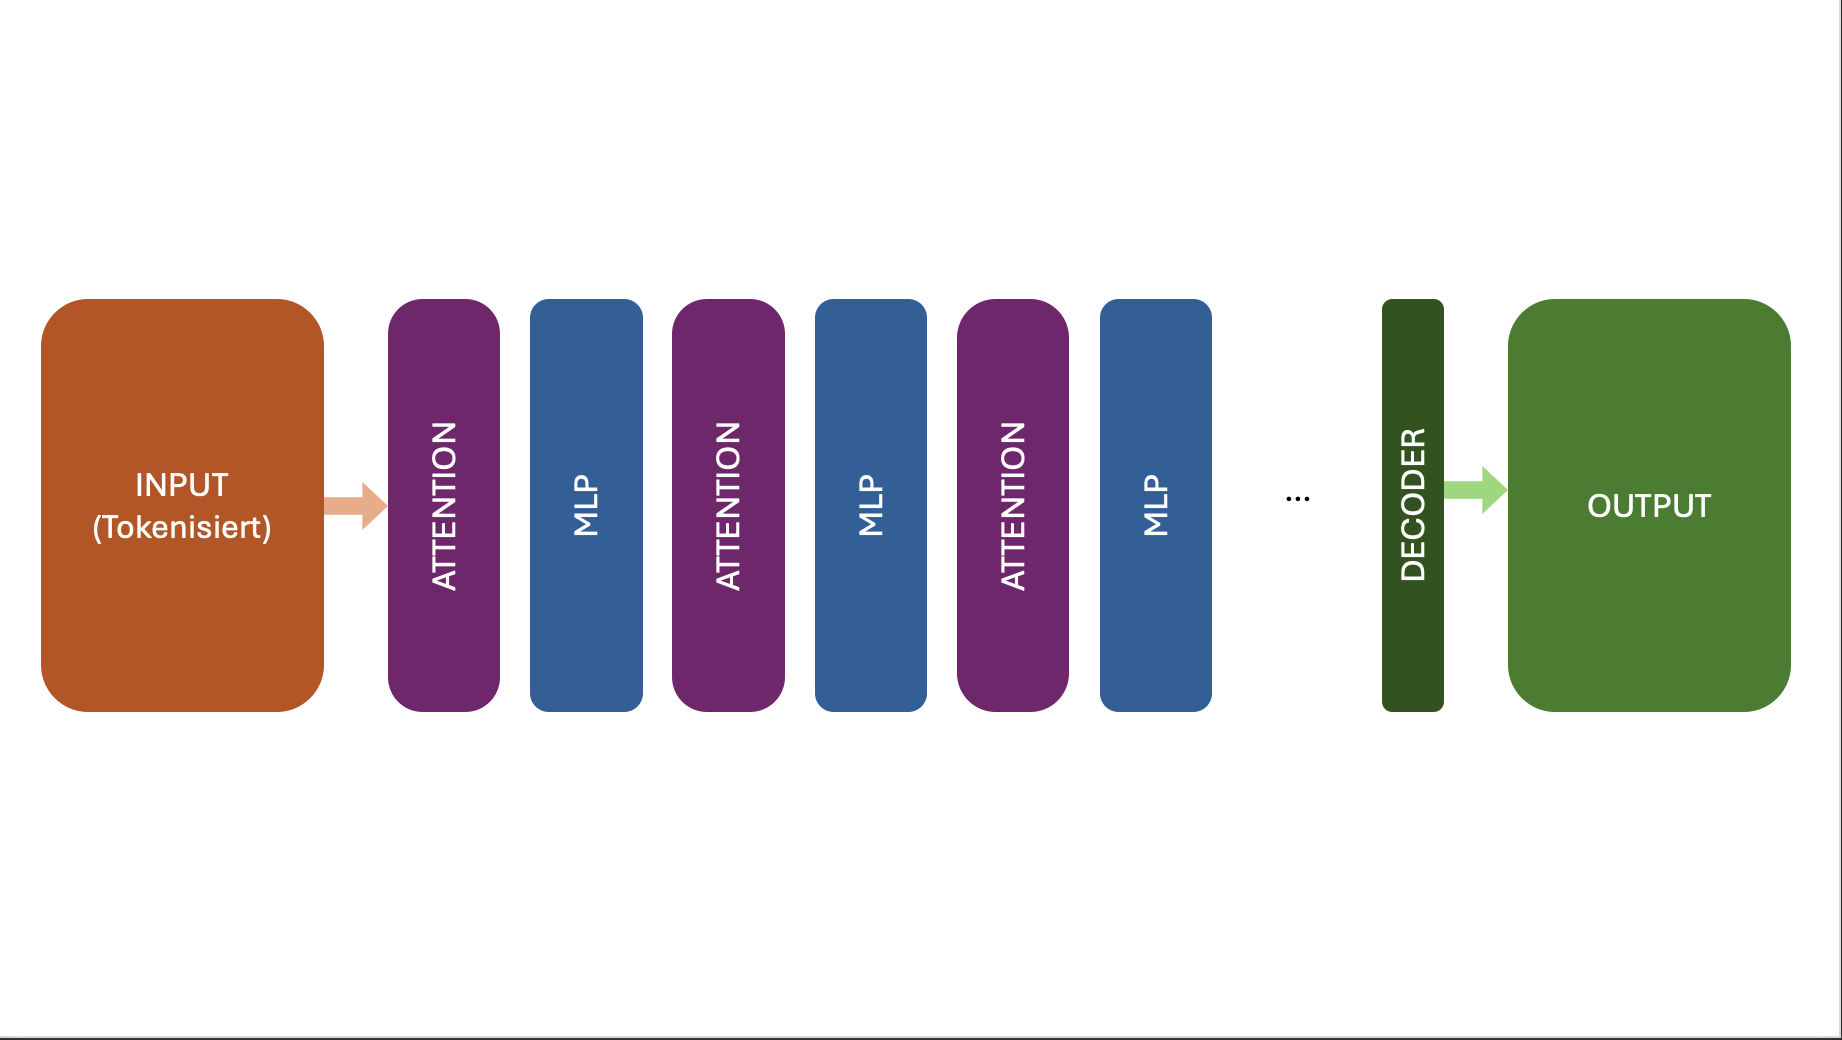
\includegraphics[scale=0.37]{bilder/Transformer.png}
  \caption{Transformer}
  \label{fig:trans}
\end{figure}

\glspl{llm} sind eine Form der \glslink{glos:ki}{KI}, die auf natürlicher Sprache basiert. Da sie entwickelt wurden, um Texte zu generieren, werden \glspl{llm} als generative 
\glslink{glos:ki}{KI} bezeichnet. Moderne \glslink{glos:llm}{LLM}s wie ChatGPT basieren auf einer Transformer-Architektur, die in Abb. \ref{fig:trans} schematisch dargestellt ist. Diese 
berechnet aus einem Eingabetext eine Wahrscheinlichkeitsverteilung über mögliche nächste Tokens. Die Transformerarchitektur besteht aus folgenden Komponenten:\cite{architecture}\\

\begin{itemize}

\item \textbf{Tokenisierung:} Zuerst wird der Eingabetext in Tokens unterteilt. Tokens können Wörter, Wortteile, Satzzeichen oder einzelne Buchstaben sein. Sie sind die kleinste Einheit, 
die das \glslink{glos:llm}{LLM} verarbeiten kann.\cite{architecture}

\item \textbf{Embedding:} Tokens werden vieldimensionalen Vektoren zugeordnet. So werden sie anhand ihrer Bedeutung codiert. Die Richtungen der Vektoren im
Vektorraum beinhalten semantische Bedeutungen. Wörter mit ähnlicher Bedeutung liegen als Vektoren im Vektorraum nahe beieinander.\cite{embedding}

\item \textbf{Attention:} Die vektorcodierten Tokens werden durch den umliegenden Text verändert, um den Wortkontext und die semantische Bedeutung widerzuspiegeln.\\
Ein Beispiel: In den Sätzen "`Ich sitze auf der Bank"' und "`Ich habe in der Bank Geld abgehoben"' erhält "`Bank"' jeweils eine andere Vektorrepräsentation, je nach Kontext liegen die codierenden 
Vektoren nahe der Tokens "`Parkbank"' oder "`Kreditinstitut"'. So bleibt der Kontext des verwendeten Wortes erhalten.\cite{attention, attention2} 

\item \textbf{\acrfull{mlp}:} Neben der linearen Attention-Funktion können mit dem \acrshort{mlp}, einem kleinen neuronalen Netzwerk mit meist nur einer inneren Schicht, auch nichtlineare Zusammenhänge 
erfasst werden. Jeder Vektor durchläuft das \acrshort{mlp}, dessen Ausgabe zum ursprünglichen Vektor addiert wird. Somit kann die Komplexität der Sprache erfasst werden.

\item \textbf{Decoder:} Ein \glslink{glos:llm}{LLM} besteht aus abwechselnden Attention- und MLP-Schichten (Abb. \ref{fig:trans}). Abschließend erhält der Decoder die Ausgabe aus der letzten 
\acrshort{mlp}-Schicht, worauf die Softmax-Funktion eine Wahrscheinlichkeitsverteilung über alle Tokens berechnet. Durch die Anwendung dieser Funktion ist die Summe der Wahrscheinlichkeiten 1 und jede liegt im Intervall zwischen 0 und 1.\cite{architecture} 
\end{itemize}

Die beschriebenen Bestandteile besitzen jeweils durch Training festgelegte Parameter. Basierend auf der sich so ergebenen Wahrscheinlichkeitsverteilung wählt das \glslink{glos:llm}{LLM} zufällig ein nächstes Wort und fügt es dem Text an. Der Vorgang wiederholt sich mit dem aktualisierten Text, 
bis eine Abbruchbedingung eintritt, etwa eine maximale Tokenanzahl oder ein spezielles Abbruchtoken.\cite{architecture}\\

\section{\gls{glos:prompt} und Kontext}

Um zu bestimmen, welchen Text das \glslink{glos:llm}{LLM} generieren soll, erhält es Eingaben, den sogenannten \gls{glos:prompt}. Da \glslink{glos:ki}{KI}-Modelle unterschiedliche Prompts 
verarbeiten können, lassen sie sich für verschiedenste Aufgaben einsetzen. Der Prompt setzt sich aus dem System-Prompt, dem User-Prompt und optional weiteren Kontextangaben zusammen.\cite{systemprompt}\\
Der System-Prompt stellt die Grundstruktur dar und gibt dem \glslink{glos:llm}{LLM} grundlegenden Kontext für die Textgenerierung mit. Zunächst erhält das Modell die Information, auf eine 
Nutzereingabe oder Frage zu reagieren, sowie die Anweisung, die Rolle des \glslink{glos:ki}{KI}-Assistenten zu übernehmen. Oft sind Stil oder Ton sowie verbotene Wörter oder Themen im System-Prompt 
enthalten. So können bereits erste Filter eingebaut werden.\cite{systemprompt} Der System-Prompt bleibt meist konstant und ist für Nutzer nicht sichtbar.\\
Der zweite Bestandteil ist der User-Prompt. Diesen gibt der Nutzer konkret ein. Wird er verändert, um das Ergebnis zu verbessern, spricht man von Prompt-Engineering. 
Dafür sind meist viele Versuche und ein tiefes Verständnis der Funktionsweise des \glslink{glos:llm}{LLM}s notwendig.\cite{promptengineering}\\
Zusätzlich zu System- und User-Prompt können weitere Informationen als Kontext übergeben werden, etwa der vorherige Chatverlauf oder relevante Texte. 
Das Kontextfenster bezeichnet die maximale Anzahl an Tokens, die dem \glslink{glos:llm}{LLM} als Eingabe mitgegeben werden können. Wird diese überschritten, kann dies zu unvollständigen 
Ergebnissen führen, da das \glslink{glos:llm}{LLM} nicht mehr alle nötgen Informationen erhält.

\section{Wirkungen und Nebenrisiken}
Mit der beschriebenen Architektur entstehen Texte, die menschengeschriebenen stark ähneln und zahlreiche Anwendungsgebiete eröffnen. Gleichzeitig ergeben sich daraus Herausforderungen und Risiken, 
die im Folgenden behandelt werden.


\subsection{Abhängigkeit von den Trainingsdaten}

Da \glslink{glos:ki}{KI} Zusammenhänge lediglich auf Grundlage der verwendeten Trainingsdaten erlernt, sind diese oft Ursache für Probleme. Werden etwa Trainingsdaten genutzt, 
bei denen bestimmte Personengruppen benachteiligt werden oder seltener vorkommen, kann dies die generierten Inhalte der \glslink{glos:ki}{KI} beeinflussen. Diskriminierende Inhalte können aus den Trainingsdaten 
übernommen werden. Zudem können fehlende Informationen über bestimmte Personengruppen, Sprachen oder Dialekte Nachteile in der Nutzung von \glslink{glos:ki}{KI} für die Betroffenen zur Folge haben.\\ 
Dieses Verhalten generativer \glslink{glos:ki}{KI} kann soziale und wirtschaftliche Folgen haben. \glslink{glos:ki}{KI}-Anbieter versuchen zwar, durch eine möglichst 
facettenreiche Auswahl von Trainingsdaten und Filtermechanismen, welche etwa das Auftreten bestimmter Wörter wie Beleidigungen verhindern, entgegenzuwirken, 
dennoch sollten sich Nutzer dieses Risikos bewusst sein.\\

\subsection{Halluzinationen}
 \glslink{glos:ki}{KI}-Halluzination beschreibt 
das Phänomen, dass generative \glslink{glos:ki}{KI}-Anwendungen scheinbar plausible, aber tatsächlich unlogische oder falsche Antworten erzeugen\cite{hallucinationForewarning}.\\
Halluzinationen können verschiedene Ursachen haben. Auch Probleme mit den Trainingsdaten sind ein häufiger Grund. Fehlen aktuelle Trainingsdaten, kann das \glslink{glos:ki}{KI}-Modell keine korrekten Aussagen zu neueren Ereignissen tätigen.\\ 
Zudem können die Daten ungenau, nicht fallspezifisch oder fehlerhaft sein, besonders wenn Trainingsdaten aus dem Internet stammen.\\ 
Schwachstellen in der Architektur sind eine weitere mögliche Ursache für Halluzinationen. Als "`Sycophancy"' wird das Phänomen bezeichnet, dass das \glslink{glos:ki}{KI}-Modell Texte 
generiert, die den Erwartungen des Nutzers entsprechen, dabei aber fachliche Korrektheit vernachlässigen. Die Formulierung des \gls{glos:prompt}s kann dies begünstigen.\cite{allgemHalluzinationen} \\
Die in \autoref{sec:llm} beschriebene Methode, mit der \glslink{glos:ki}{KI} Texte erzeugt, birgt ebenfalls ein Risiko für Falschinformationen. Ein Artikel des Frauenhofer-Instituts beschreibt, dass manche Token-Typen sehr nah beieinander liegen 
und ähnliche Wahrscheinlichkeiten haben. Dazu zählen "`ähnliche numerische Werte wie Preise (9,99 EUR; 10,00 EUR), nahe beieinander liegende Daten (2020, 2021), ähnlich klingende Namen oder 
technische Begriffe und Abkürzungen (\glslink{glos:ki}{KI}, ML)"'\cite{halluzinationenFraunhofer}. Die Verwechslung solcher Daten kann leicht zu fehlerhaften Aussagen führen.\\
Bei der Auswahl des nächsten Tokens können durch die Wahrscheinlichkeitsberechnung, wie in \autoref{sec:llm}  beschrieben, unpassende Wörter bevorzugt werden, die wiederum Halluzinationen 
begünstigen. Technisch lässt sich dies mit dem sogenannten Softmax-Bottleneck erklären: Der Softmax-Algorithmus kann mit seiner Natur nur einen Ausschnitt aller möglichen 
Wahrscheinlichkeitsverteilungen darstellen, sodass manche Verteilungen nicht exakt abgebildet werden und unpassende Wörter eine zu hohe Wahrscheinlichkeit bekommen.\cite{softmax} \\
Ein einmal falsch gewähltes Wort, welches dem Text angefügt wird, bildet wiederum die Grundlage für die nächsten generierten Wörter. Tritt eine bestimmte Falschinformation auf, 
kann "`Over-Confidence"' dazu führen, dass trotz Nachfragen oder Korrekturversuchen das \glslink{glos:ki}{KI}-Modell weiterhin auf die falsche Behauptung besteht. Dies erschwert die 
Überprüfung für den Anwender.\cite{allgemHalluzinationen,softmax} \\
Selbst wenn ein \glslink{glos:ki}{KI}-Text keine Falschinformationen enthält, können diese Phänomene Unvollständigkeit oder ein Abweichen von der Fragestellung bewirken. Das als 
"`Instructions-Forgetting"' bekannte Phänomen beschreibt, dass eine \glslink{glos:ki}{KI} den Kontext der ursprünglichen Anfrage vergisst und einen Text generiert, der von der 
eigentlichen Fragestellung abweicht. Daher sollten \glslink{glos:ki}{KI}-generierte Texte, besonders beim wissenschaftlichen Schreiben, immer überprüft werden.\cite{allgemHalluzinationen}


\subsection{Erklärbarkeitsproblem}
\label{sec:erklärbarkeitsproblem}

Das Erklärbarkeitsproblem adressiert die Schwierigkeit, die Begründung für spezifische Entscheidungen der \glslink{glos:ki}{KI} nachvollziehbar zu machen. Aufgrund der Funktionsweise nach dem sogenannten 
"`Black-Box"'-Prinzip ist die Rekonstruktion der kausalen Faktoren, die zu einem bestimmten Ergebnis geführt haben, limitiert. Diese Intransparenz kann die Akzeptanz und das Vertrauen in 
KI-basierte Entscheidungen beeinträchtigen. Darüber hinaus erschwert sie die Identifizierung und Korrektur von Fehlern in der zugrundeliegenden Architektur. Aktuelle Forschungsansätze 
im Bereich der "`erklärbaren KI"' zielen darauf ab, dieses Problem zu adressieren, indem sie beispielsweise Mechanismen zur Visualisierung und Darstellung des 
Entscheidungsfindungsprozesses entwickeln.\cite{explainable}
 

\subsection{Ressourcenverbrauch}

KI-Modelle verbrauchen während des Trainings und beim Bearbeiten von Anfragen viele Ressourcen. Desto größer das verwendete Modell, desto höher ist der Ressourcenverbrauch. 
Der Stromverbrauch von GPT4 liegt laut eines im Jahr 2025 veröffentlichten Artikels bei bis zu einer Kilowattstunde pro Anfrage\cite{Energieverbrauch}. Für die oben beschriebene Anpassung der Parameter sind während des Bearbeitens einer Anfrage viele 
komplexe Berechnungen in möglichst kurzer Zeit notwendig. Auch das Training ist durch die große Menge benötigter Daten und die häufig wochen- bis monatelangen Trainingszeiten 
energieintensiv. In den Rechenzentren wird zudem Wasser zur Kühlung verwendet. Der Wasser-und Ressourcenverbrauch der Nutzung eines \glslink{glos:ki}{KI}-Modells ist im Vergleich zu dem der Nutzung einer 
Suchmaschine wie Google sehr hoch\cite{KINachhaltigkeit}. 

\subsection{Datenschutz}
\label{sec:datenschutz}

Des Weiteren besteht bei dem Training sowie bei der Nutzung von \glslink{glos:ki}{KI} das Problem des Datenschutzes. Die Trainingsdaten können personenbezogene Informationen beinhalten, welche ungewollt 
wiedergeben werden können. Einige \glslink{glos:llm}{LLM}-Anbieter behalten sich das Recht vor, das Modell anhand der 
Eingabedaten weiter zu trainieren und die Daten anderweitig zu nutzen\cite{OpenAI_Datenschutzerklaerung_2025,MistralAI_Terms_2025}. Auch so können personenbezogenen oder unternehmensspezifischen Informationen in die Trainings- oder Ausgabedaten 
erscheinen und so zu Datenschutzverletzungen führen.\\ Im Falle einer missbräuchlichen Verwendung solcher Daten ist oft unklar, wer dafür die Verantwortung trägt. Vor allem bei der \glslink{glos:ki}{KI}-Nutzung 
über Online-Schnittstellen sollte daher sorgfältig mit wichtigen Informationen umgegangen werden. Sie sollten beispielsweise nicht in Form des \gls{glos:prompt}s an das Modell gegeben werden.


\end{document}